\documentclass{article}
%packages
\usepackage{graphicx}
\usepackage[utf8]{inputenc}
\usepackage[T1]{fontenc}
\usepackage[frenchb]{babel}
\usepackage[margin=0.5in]{geometry}

\begin{document}
%title
\begin{titlepage}
	\vspace{-20px}
	\begin{tabular}{l}
		\textsc{Blin} S\'ebastien\\
		\textsc{Collin} Pierre-Henri
	\end{tabular}
	\hfill \vspace{10px}
\includegraphics[scale=0.1]{esir.png}\\
	\vfill
	\begin{center}
		\Huge{\'Ecole sup\'erieure d'ing\'enieurs de Rennes}\\
		\vspace{1cm}
		\LARGE{1\`ere Ann\'ee}\\
		\large{Parcours Informatique}\\
		\vspace{0.5cm}\hrule\vspace{0.5cm}
		\LARGE{\textbf{BDD}}\\
		\Large{Compte-Rendu Mixage}
		\vspace{0.5cm}\hrule
		\vfill
		\vfill
	\end{center}
	\begin{flushleft}
		\Large{Sous l'encadrement de~:}\\
		\vspace{0.2cm}
		\large{{Lamarche} Fabrice}
	\end{flushleft}
	\vfill
\end{titlepage}

\section{Diagramme de classe}
\begin{figure}
	\begin{center}
		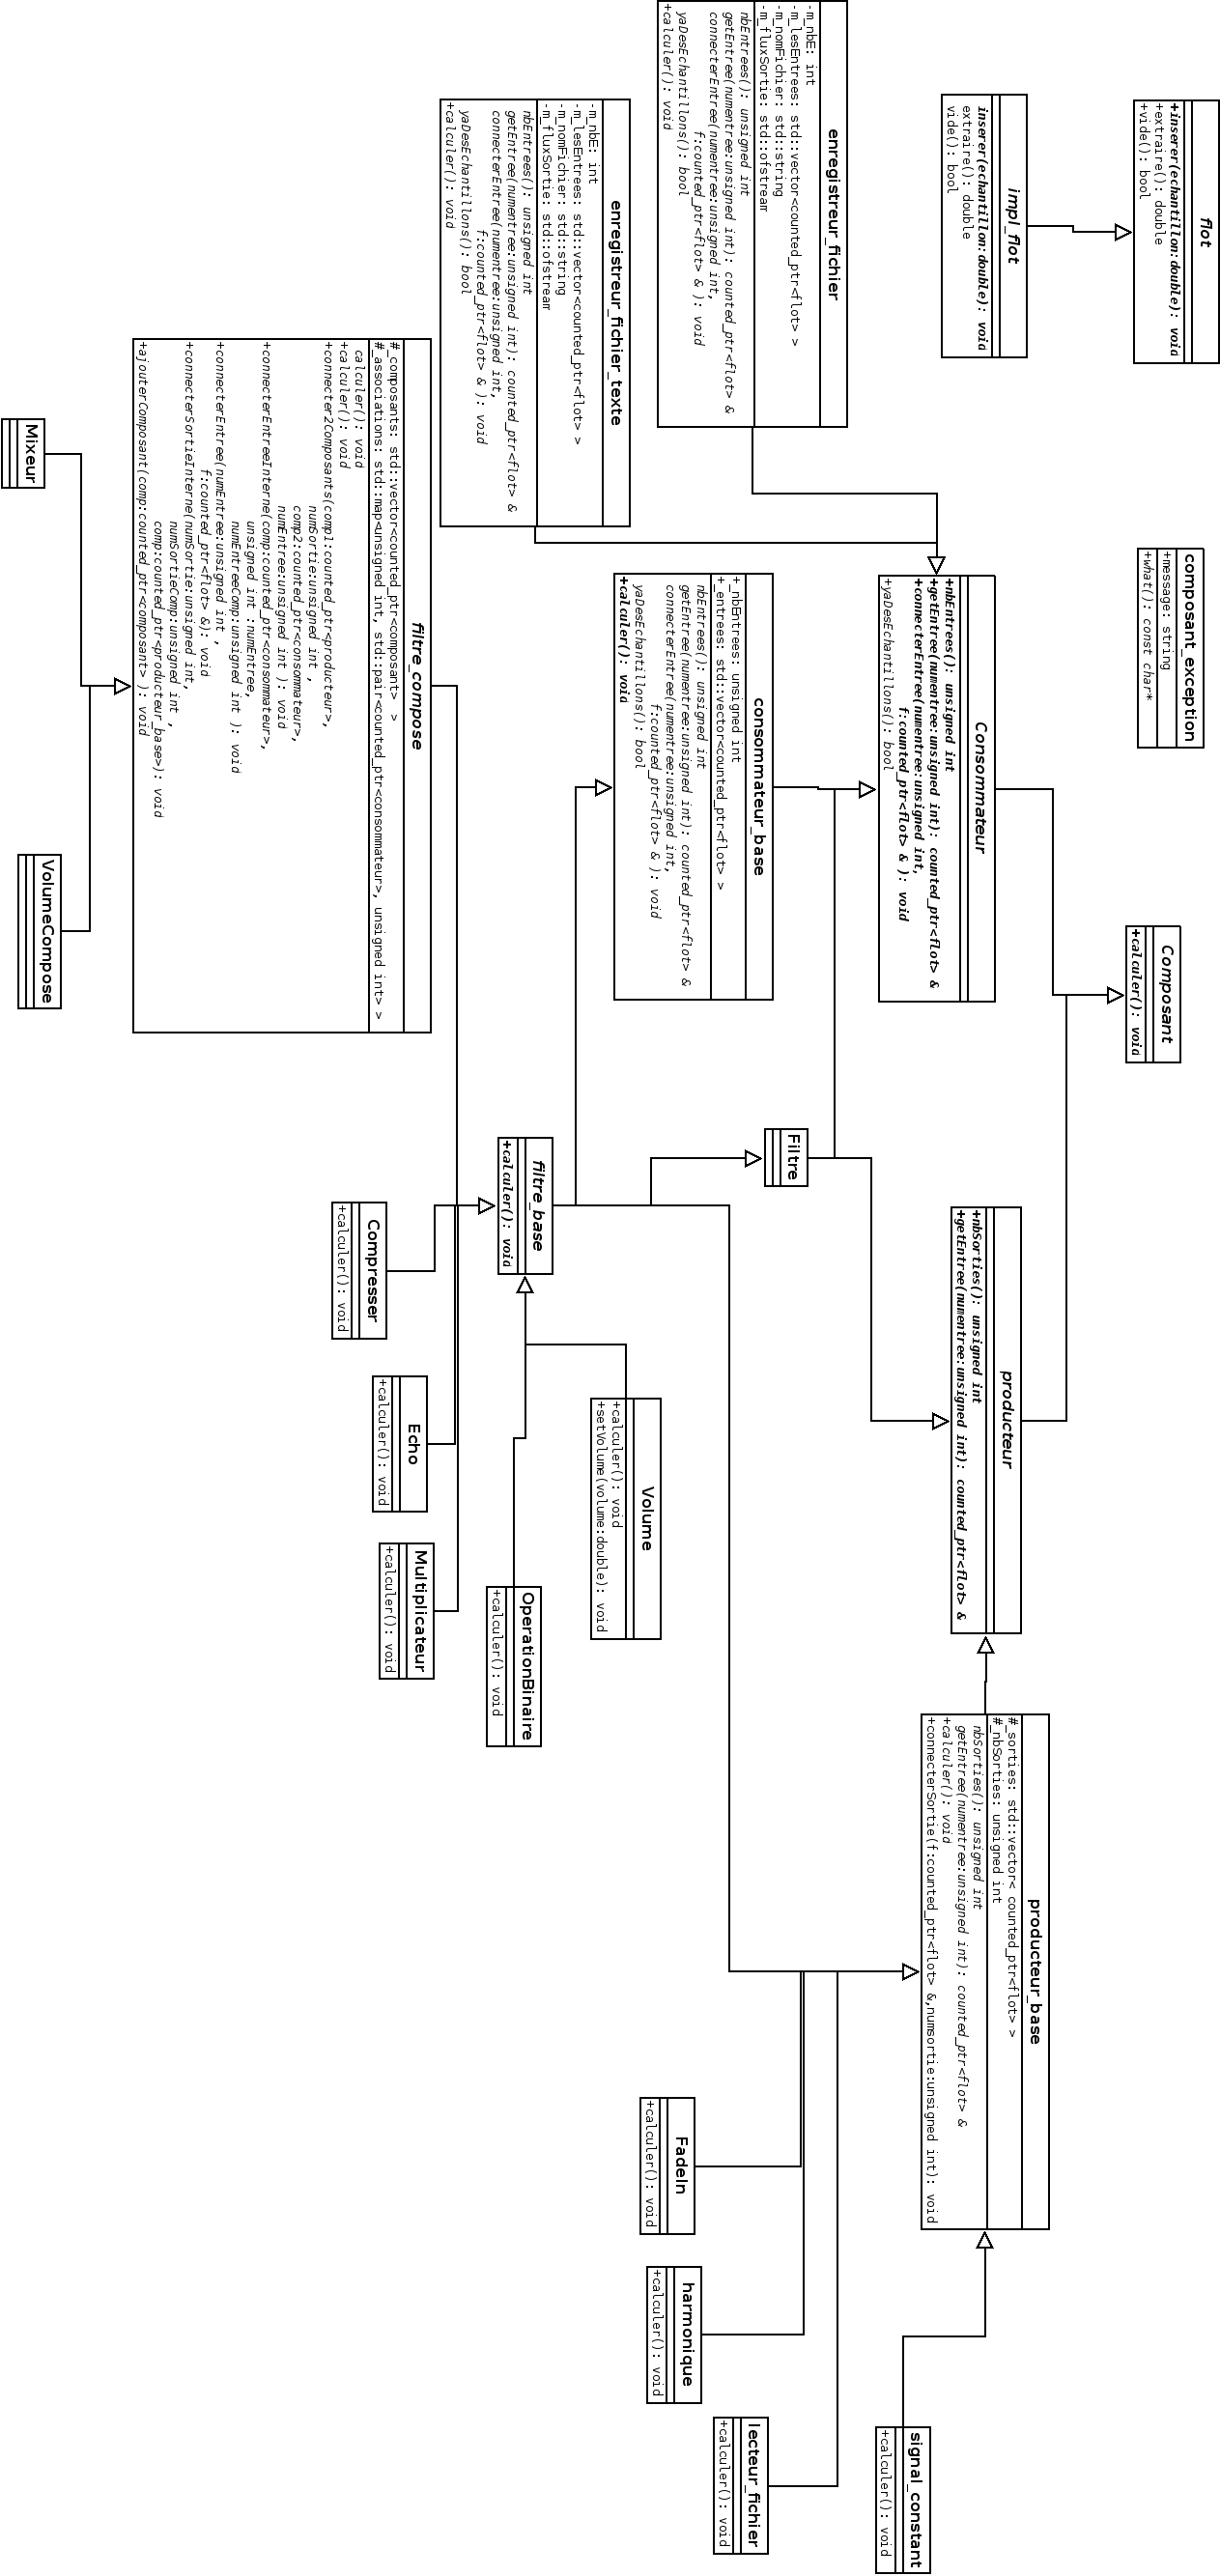
\includegraphics[scale=0.25]{TP13}\\
		Diagramme de classe
	\end{center}
\end{figure}

\section{Filtres composés}
Le filtre composé est un filtre contenant plusieurs objets héritants de composant.\\
Ils sont stockés dans std::vector<counted\_ptr<composant>  > \_composants;\\
Pour garder en mémoire les connexions entre les entrées du filtre et les composants internes, une map est nécessaire. Ces données sont contenus dans : \\
std::map<unsigned int, std::pair<counted\_ptr<consommateur>, unsigned int> > \_associations;\\
Modifiée par void connecterEntreeInterne (counted\_ptr<consommateur> comp, unsigned int numEntree, unsigned int numEntreeComp);\\
Les connexions entre composants se font via la méthode void connecter2Composants(counted\_ptr<producteur> comp1, unsigned int numSortie,	counted\_ptr<consommateur> comp2, unsigned int numEntree);\\

\begin{figure}
	\begin{center}
		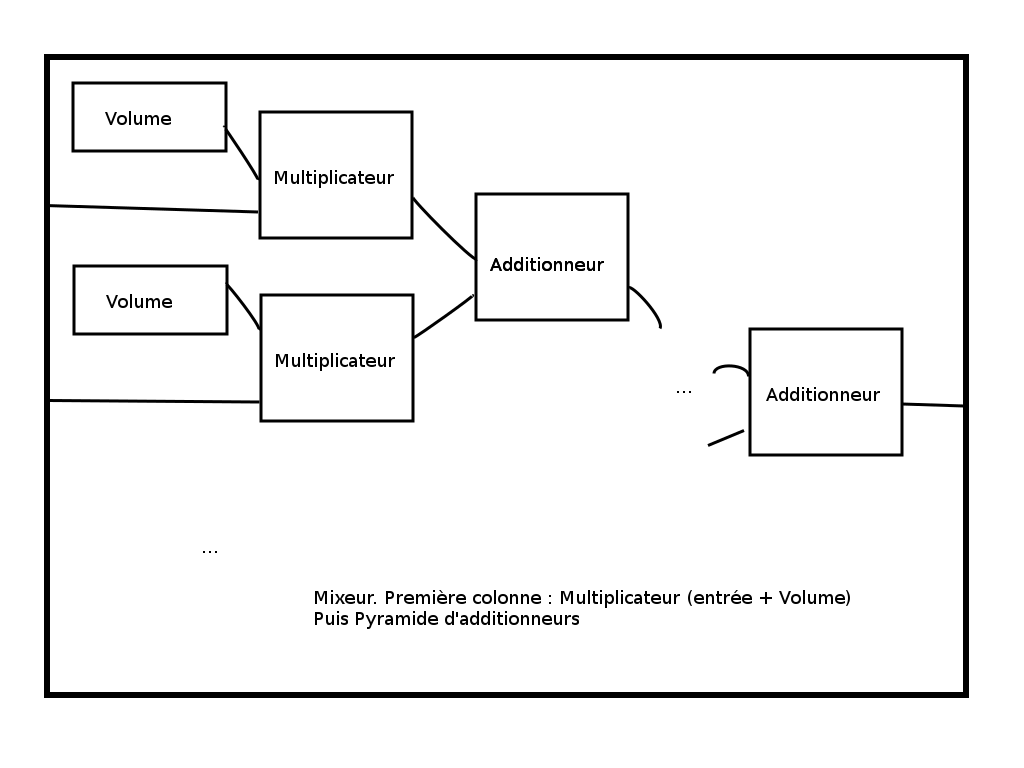
\includegraphics[scale=0.25]{mixeur}\\
		Mixeur
	\end{center}
\end{figure}

\begin{figure}
	\begin{center}
		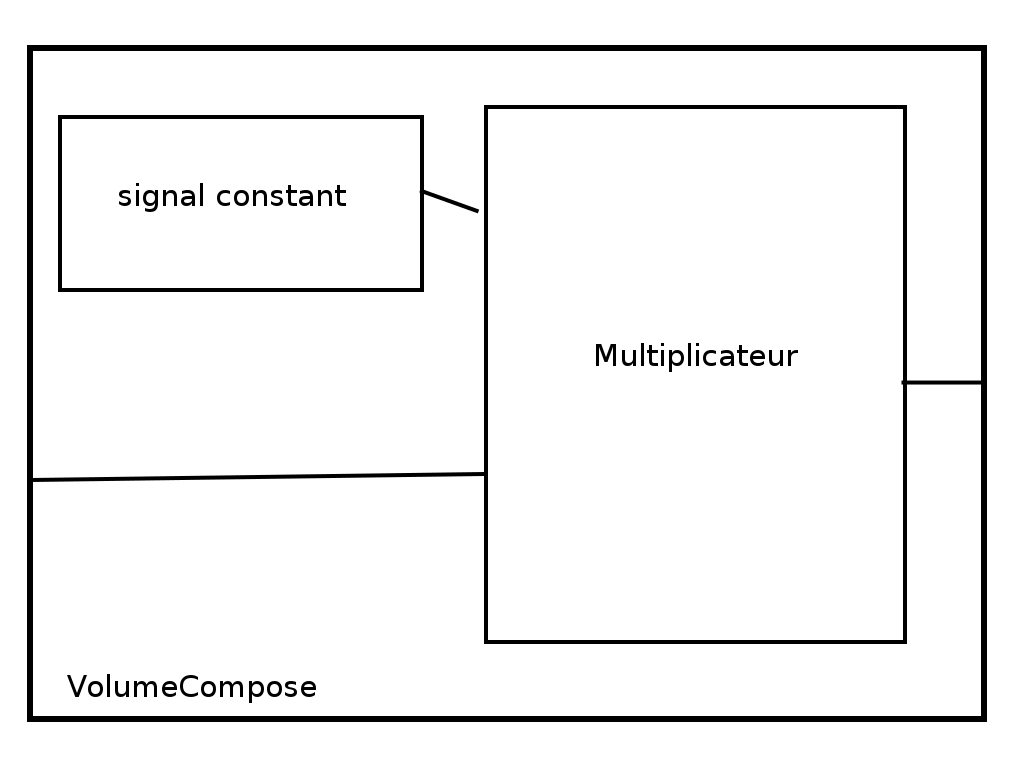
\includegraphics[scale=0.25]{volumeCompose}\\
		Volume composé
	\end{center}
\end{figure}


\end{document}
